\section{Theoretical Framework}
Before establishing the technical implementation of a scalable smart gardening system, a conceptual foundation must be established. Designing an IoT infrastructure involves significant complexity, and standardized reference models are essential for organizing this architecture. This section analyzes required IoT models and explores modern cloud solutions, particularly Backend-as-a-Service (BaaS) platforms. These theoretical components are critical for evaluating the design choices implemented in Plant Up!.

\subsection{The IoT World Forum Reference Model (7-Layer Model)}

Analyzing a large-scale, distributed IoT architecture requires a clear structural framework. This thesis utilizes the IoT World Forum 7-Layer Reference Model, which provides a holistic view encompassing physical hardware, connectivity, and cloud services. This model serves as the baseline for differentiating between Edge (or Fog) and Cloud computing \cite{iot_reference_model}.

The model categorizes the ecosystem into seven layers. Layers 1 and 2 (Physical Devices and Connectivity) address edge hardware, sensors, and the network protocols for data transmission. Layer 3 (Edge Computing) involves local processing to minimize latency by handling data close to the source. Layers 4 and 5 (Data Accumulation and Abstraction) manage data buffering and transformation in the cloud, while Layers 6 and 7 (Application and Collaboration) execute business logic and facilitate user interaction.

\begin{figure}[htbp]
    \centering
    \scalebox{1.3}{\IoTNavigator{0}{1}}
    \caption{The 7-Layer IoT World Forum Reference Model (Unified Visual Representation)}
    \label{fig:iot_reference_model}
\end{figure}

A central focus of this thesis is the distribution of decision-making logic between local hardware (Layer 3) and centralized cloud services (Layers 5 and 6). The 7-layer model establishes the boundaries necessary for analyzing this computational separation.

\subsection{Modern IoT Backends}
IoT backends must simultaneously handle diverse workloads, including structured relational data (e.g., user accounts) and high-velocity sensor streams. This section explores Backend-as-a-Service (BaaS) platforms and specialized database extensions designed to manage these workloads without requiring manual infrastructure orchestration.

\subsubsection{Backend-as-a-Service (BaaS) and the SQL vs. NoSQL Paradigm}

Backend-as-a-Service (BaaS) provides developers with managed infrastructure, including databases, authentication, and serverless APIs. While early BaaS platforms frequently utilized NoSQL document stores (such as Firebase), these architectures can face challenges with complex analytical queries and relational integrity in advanced IoT ecosystems \cite{closefuture_supabase_firebase, supabase_alternatives}. 

Modern BaaS architectures often utilize Relational Database Management Systems (RDBMS), such as PostgreSQL, which provide data integrity alongside real-time subscription capabilities for mobile clients \cite{blog_elest_supabase_self_host}.

\begin{figure}[htbp]
    \centering
    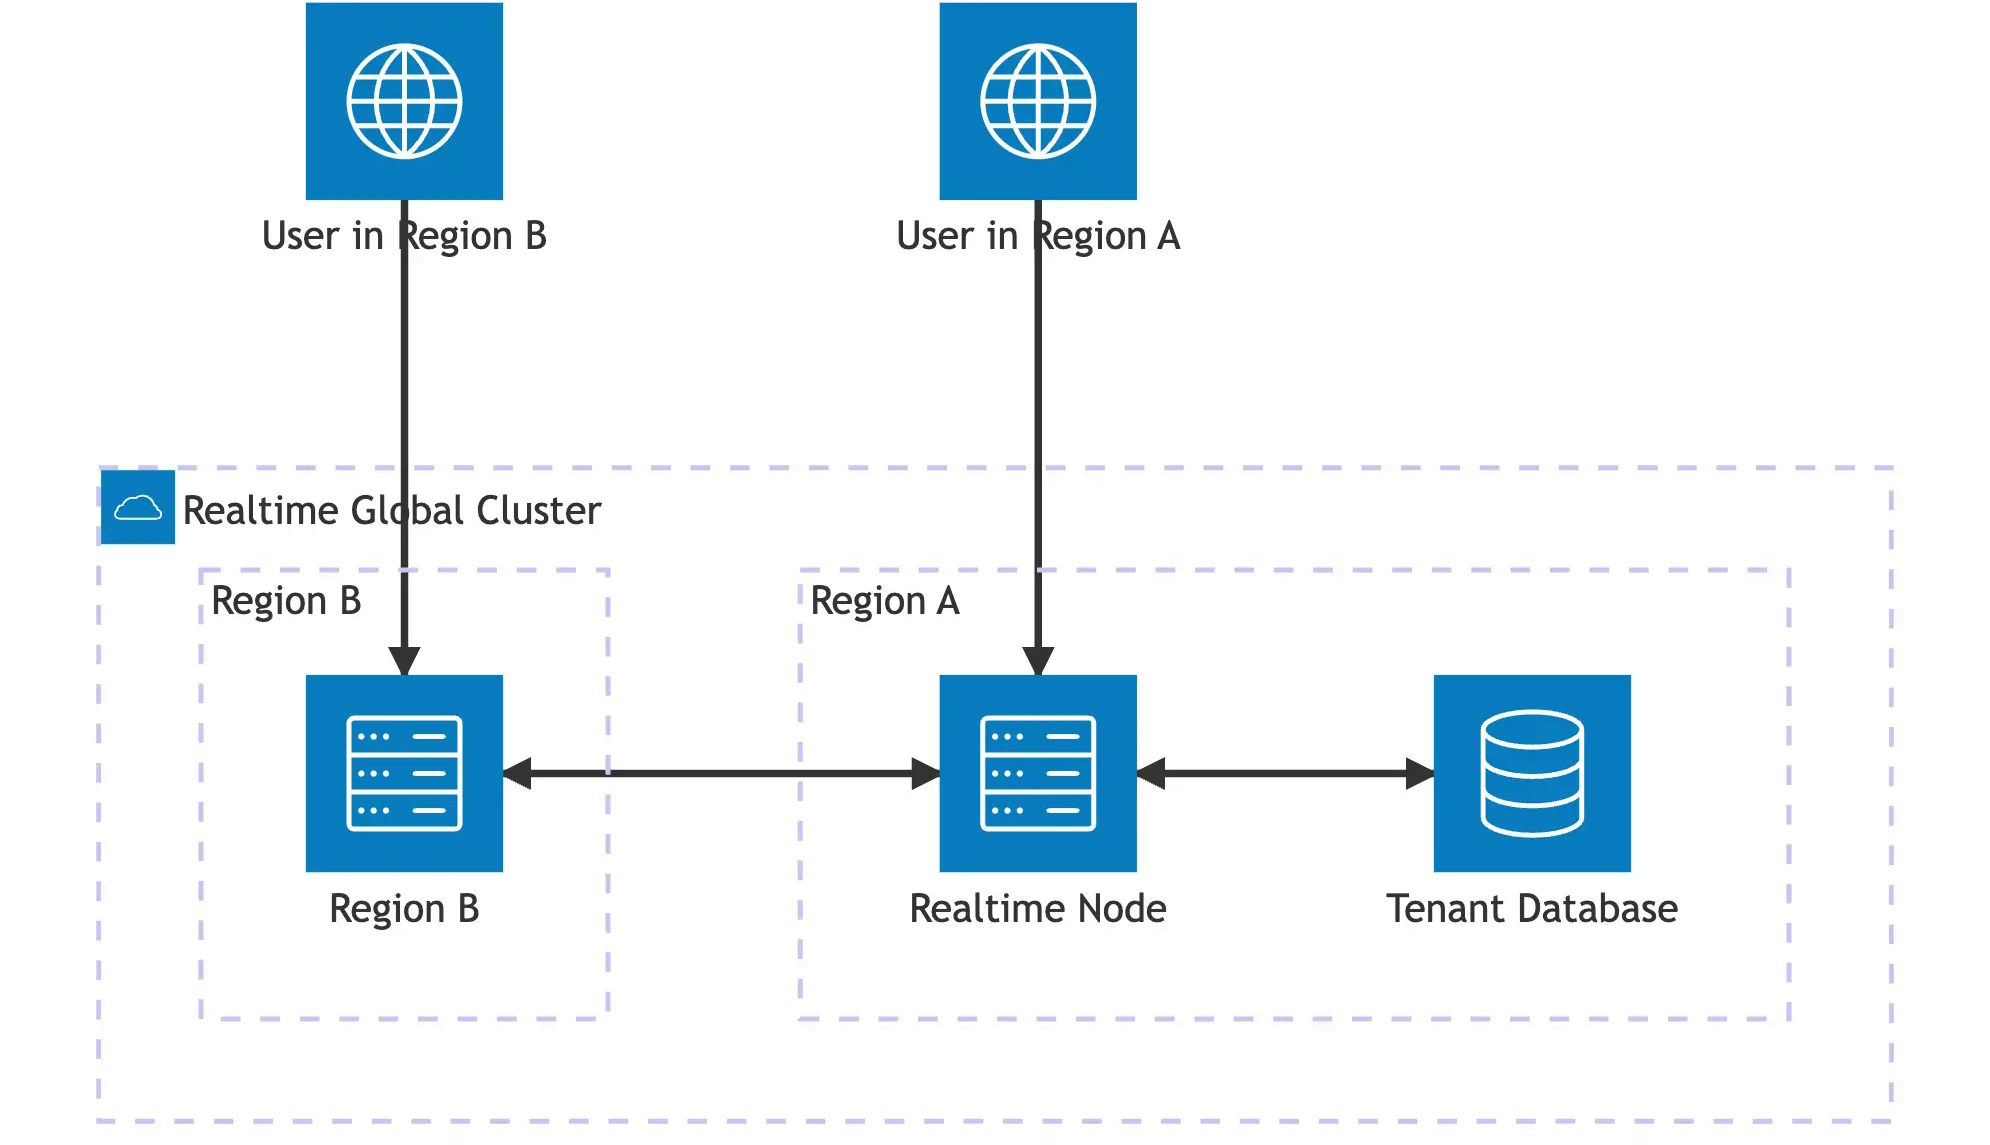
\includegraphics[width=0.8\textwidth,height=0.45\textheight,keepaspectratio]{Abudi/figures/realtime_architekture.png}
    \caption{Real-time Architecture Flow in Modern BaaS \cite{realtime_architecture}}
    \label{fig:realtime_architecture}
\end{figure}

When selecting a BaaS for an IoT ecosystem, extensibility is a critical factor. While standard relational databases ensure transactional consistency (ACID properties), they may require optimization to handle high-velocity sensor streams. Consequently, a BaaS is often enhanced with specialized extensions, such as time-series modules, to optimize the SQL engine for sensor data ingestion \cite{closefuture_supabase_firebase, blog_elest_supabase_self_host}.

\subsubsection{Time-Series Databases: Challenges with Standard SQL for Sensor Streams}

Traditional relational databases, while effective for standard transactional workloads, can experience performance issues when managing high-velocity IoT sensor streams \cite{tigerdata_tsdb_vs_rdbms}. A primary cause is index degradation. 

Standard B-tree indexes can become resource-intensive to maintain as table sizes increase with continuous telemetry data. High ingestion rates can lead to significant RAM consumption by the index, potentially impacting read query performance and server stability. To address this, specialized time-series extensions are implemented to replace standard indexing with time-based partitioning \cite{milvus_rdbms_limitations}.

\subsubsection{The TimescaleDB Extension: Hypertables and Chunking}
Standard relational databases often struggle with the sheer volume of incoming sensor data, but the TimescaleDB extension solves this by transforming PostgreSQL into a dedicated time-series engine while keeping the standard SQL interface. The core of this optimization is the use of "hypertables," which appear as normal tables to the developer but are actually partitioned into smaller physical "chunks" sorted by time intervals, such as days or weeks \cite{tigerdata_tsdb_compared, tigerdata_best_practices_hypertables, tigerdata_timescale_alternatives, tigerdata_caggs_retention}. This approach exploits the fact that most IoT queries target recent data; by directing inserts into only the active chunk, the system avoids scanning through massive amounts of historical logs, which keeps ingestion fast and range queries responsive even as the dataset grows. To further reduce the load, TimescaleDB supports continuous aggregates that precompute summaries like hourly averages in the background, alongside retention policies that automatically compress or purge old data to save space \cite{tigerdata_best_practices_hypertables, tigerdata_timescale_alternatives, tigerdata_caggs_retention, tigerdata_tsdb_compared}. Ultimately, this chunked architecture reduces the I/O and indexing pressure that usually bogs down standard tables, as shown in Figure \ref{fig:hypertable_vs_normal}, providing a high-performance solution that doesn't sacrifice SQL compatibility.

\begin{figure}[htbp]
    \centering
    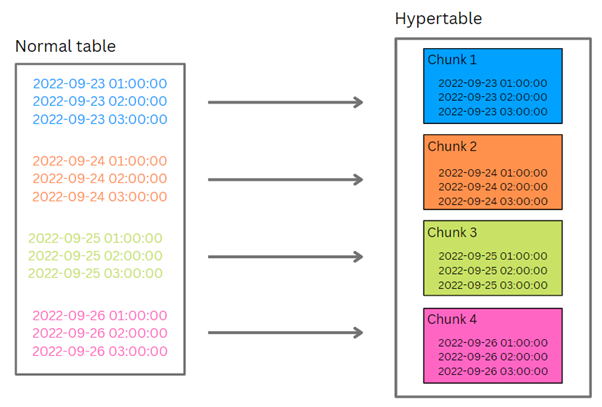
\includegraphics[width=0.8\textwidth,keepaspectratio]{Abudi/figures/HyperTableVSNormal.png}
    \caption{Architectural comparison between a standard PostgreSQL table and a TimescaleDB hypertable with chunked storage.}
    \label{fig:hypertable_vs_normal}
\end{figure}


\subsection{Microservices in IoT}

As IoT systems expand, monolithic architectures, where all features are integrated into a single unit, can present challenges for stability and maintenance. 

To ensure stability and development efficiency, modern scalable architectures often utilize microservices. This approach partitions system functionality into focused, independent services. Adopting microservices allows for the separation of external device communication, including MQTT brokers, from user-facing features, facilitating clearly defined interfaces and modularity \cite{microservices_io_gateway}.

\subsubsection{The Gateway Pattern: Bridging Edge and Core Services}
Connecting an ESP32 directly to a database presents a significant security risk, as hardcoding API keys into firmware makes them vulnerable if a device is ever compromised. The Gateway pattern addresses this by acting as a secure boundary and protocol translator between the physical hardware and the core backend \cite{microservices_io_gateway, microservices_io_patterns, microservices_io_apigateway}. In this architecture, sensors push data to a message broker, and the Gateway service—housed within a secure cloud network—processes these messages for database insertion \cite{microservices_io_apigateway}. This separation maintains security while allowing backend logic updates without modifying firmware on deployed devices. It also facilitates scaling by regional brokers to funnel data into a central instance without causing bottlenecks \cite{digitalapi_gateway_pattern, microservices_io_apigateway}. By validating and structuring all incoming traffic, the Gateway ensures the core system remains modular and protected from the intricacies of edge communication \cite{microservices_io_apigateway}.

\subsubsection{Service Inter-communication: Synchronous vs. Asynchronous Patterns}
Inter-service communication is fundamental to system reliability, particularly in high-volume sensor networks. Synchronous configurations, such as standard HTTP requests, require services to wait for responses, which often leads to cascading delays when network traffic increases \cite{gfg_microservices_communication}. To mitigate this risk, scalable IoT architectures frequently utilize asynchronous, event-driven communication. In this model, a service publishes a message to a broker and continues processing without waiting for a reply \cite{gfg_sync_vs_async_system_design}. This approach enhances architectural resilience; for instance, if a large number of devices reconnect simultaneously, an asynchronous Gateway can queue the incoming traffic, allowing the database to process data at a sustainable rate \cite{cerbos_inter_service_communication}.

\subsection{Edge vs. Cloud}
The allocation of computational logic is a critical design choice in IoT engineering, typically falling on a spectrum between the cloud and the edge. In a cloud-centric model, edge hardware acts as a "thin" component that exclusively transmits data to remote servers for processing \cite{digitalocean_edge_vs_cloud, blog_elest_supabase_self_host}. While this centralizes computing power for tasks like complex time-series aggregations, it creates a dependency on stable network connectivity and introduces potential latency \cite{nsf_par_10184999, gfg_cloud_computing}. Conversely, an edge-centric approach places decision-making logic directly on the microcontroller, providing localized autonomy and low latency as shown in Figure \ref{fig:cloud_vs_edge}. This model enables rapid responses and offline fault tolerance, though it is constrained by limited hardware resources and increased maintenance complexity \cite{scalecomputing_edge_vs_cloud, scalecomputing_edge_devices, blog_elest_supabase_self_host}. Balancing these factors through "Thick" or "Thin" edge strategies is essential for ensuring that systems like Plant Up! remain both analytically capable and operationally resilient.

\begin{figure}[htbp]
    \centering
    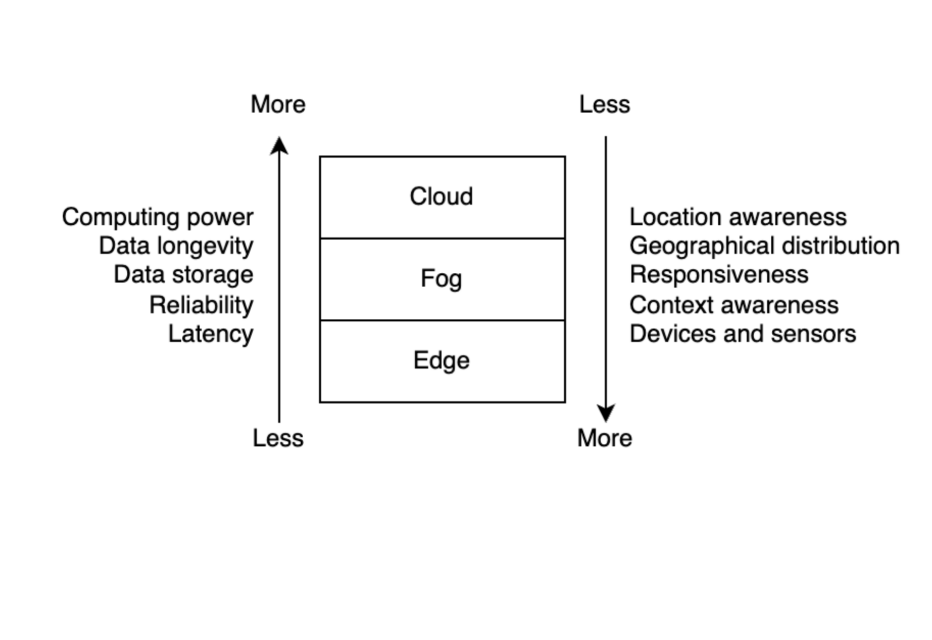
\includegraphics[width=0.8\textwidth]{Abudi/figures/cloud vs edge.png}
    \caption{Visual Comparison of Cloud vs. Edge Architectures.}
    \label{fig:cloud_vs_edge}
\end{figure}
are evaluated.
